\documentclass{beamer}
\usepackage{nameref}
\usetheme{Madrid}
\graphicspath{ {./images/} }

\begin{document}
	
	\title{Gestione centraline elettriche}
	\subtitle{Architettura del software}
	\author{Michele Beccari 856608}
	\date{2024}
	
	\begin{frame}
		\titlepage
	\end{frame}

	\begin{frame}{Indice}
		\tableofcontents
	\end{frame}
	
	
	\section{Obbiettivo del progetto}\label{obbiettivo}
	
	\begin{frame}
		\frametitle{\nameref{obbiettivo}}
		\begin{block}{\nameref{obbiettivo}}
			Si vuole realizzare un sistema per la GEstione di Centraline (GEC) di distribuzione di energia elettrica. \\
			Le centraline sono sparse sul territorio e sono dotate di sensori per la misura istantanea della potenza erogata. \\
			Il sistema deve essere in grado di gestire le anomalie nell'erogazione della potenza delle centraline. \\
			In caso di guasti il sistema deve consentire al servizio tecnico centrale l'invio di un operatore adatto alla risoluzione del guasto.
		\end{block}
	\end{frame}
	
	\section{Assunzioni}\label{assunzioni}
	
	\begin{frame}
		\frametitle{\nameref{assunzioni}}
			\begin{block}{Centraline}
				\begin{itemize}
					\item Sono connesse ad internet
					\item Sono dotate di un sistema che ne riceve i dati del sensore ed è in grado di comunicare i dati al servizio tecnico centrale
					\item Possono essere di diverse tipologie
				\end{itemize}
			\end{block}
			\begin{block}{Guasti}
					\begin{itemize}
						\item Ad ogni anomalia viene assegnato un unico operatore per la risoluzione.
					\end{itemize}
			\end{block}
			\begin{block}{Operatori}
				\begin{itemize}
					\item Ogni operatore è in grado di operare su una o più tipologie di centraline.
				\end{itemize}
			\end{block}
	\end{frame}
	
	\section{Terminologia}\label{terminology}
	
	\begin{frame}
		\frametitle{\nameref{terminology}}
		\begin{block}{Datastore}
			\begin{itemize}
				\item DALC: datastore letture centraline.
			\end{itemize}
		\end{block}
		\begin{block}{Buffer}
			\begin{itemize}
				\item BALC: buffer letture centraline.
			\end{itemize}
		\end{block}
	\end{frame}

	\section{Architettura del problema}\label{arch_problema}
	
	
	\subsection{Modello di dominio}\label{domain_model}
	\begin{frame}
		\frametitle{\nameref{domain_model}}
		\begin{center}
			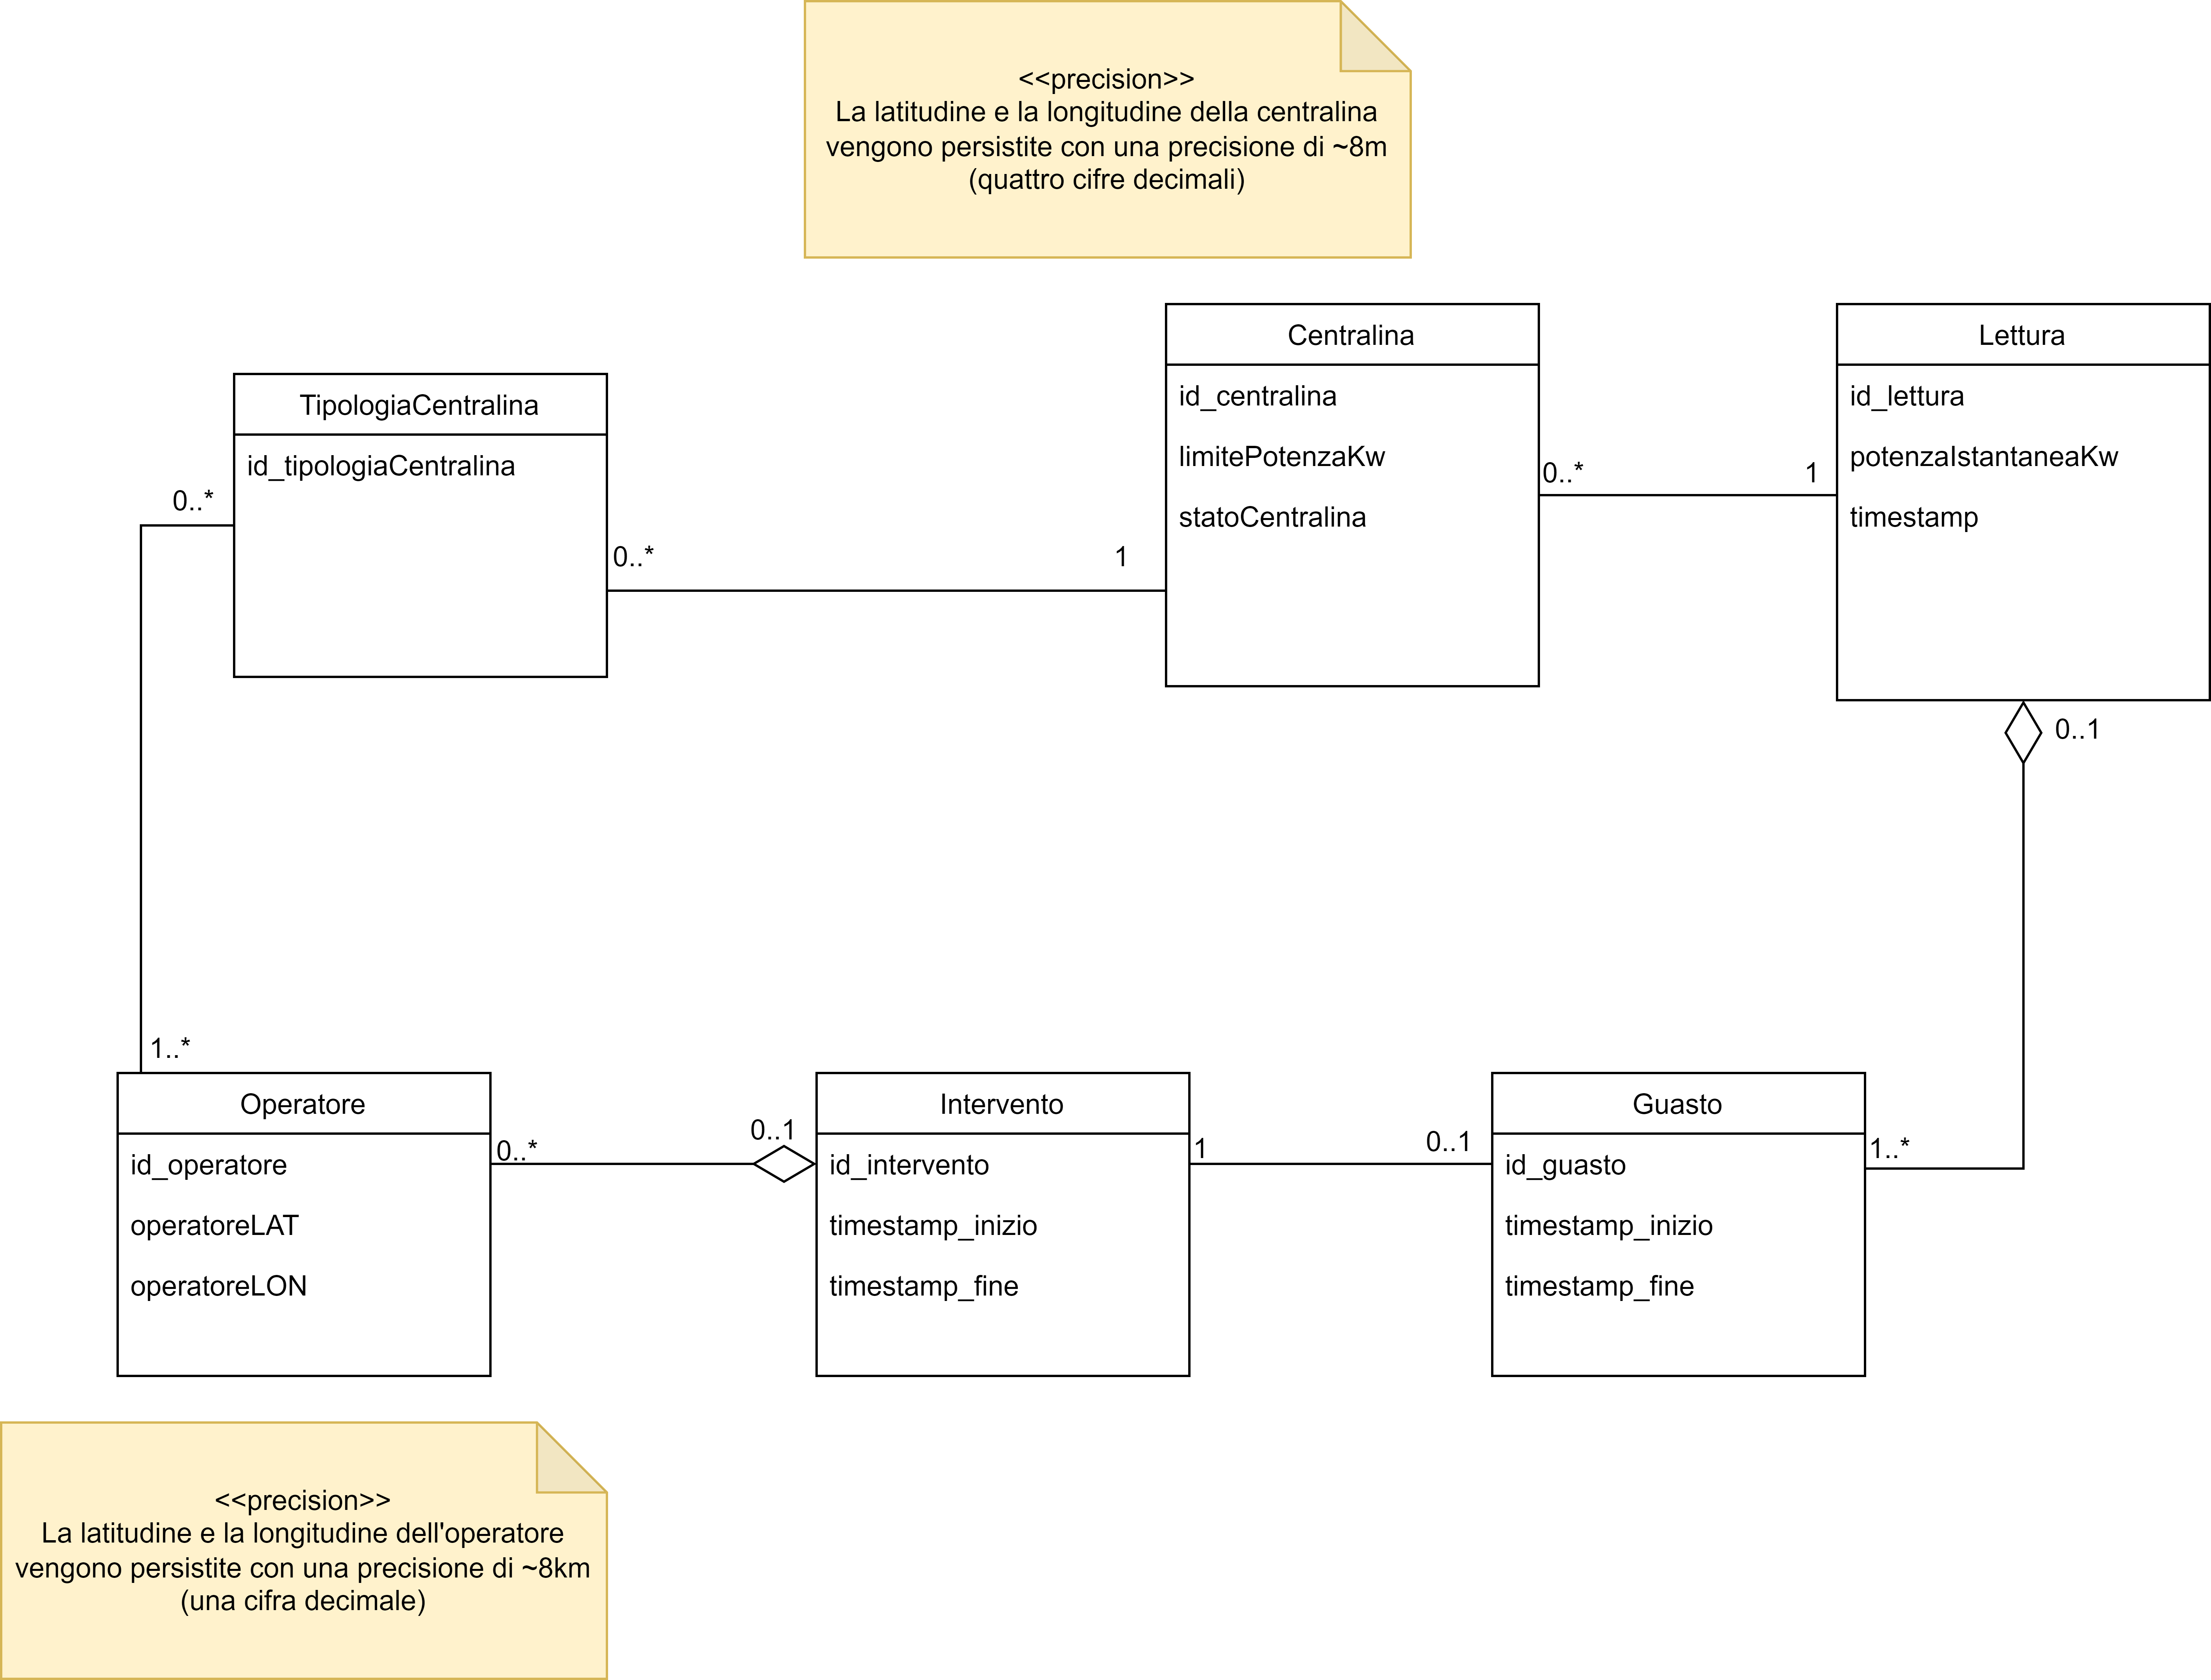
\includegraphics[width=0.85\textwidth, height=\textheight, keepaspectratio=true]{domain_model.png}
		\end{center}
	\end{frame}
	
	\subsection{Diagramma dei casi d'uso}\label{use_cases_diagram}
	\begin{frame}
		\frametitle{\nameref{use_cases_diagram}}
		\begin{center}
			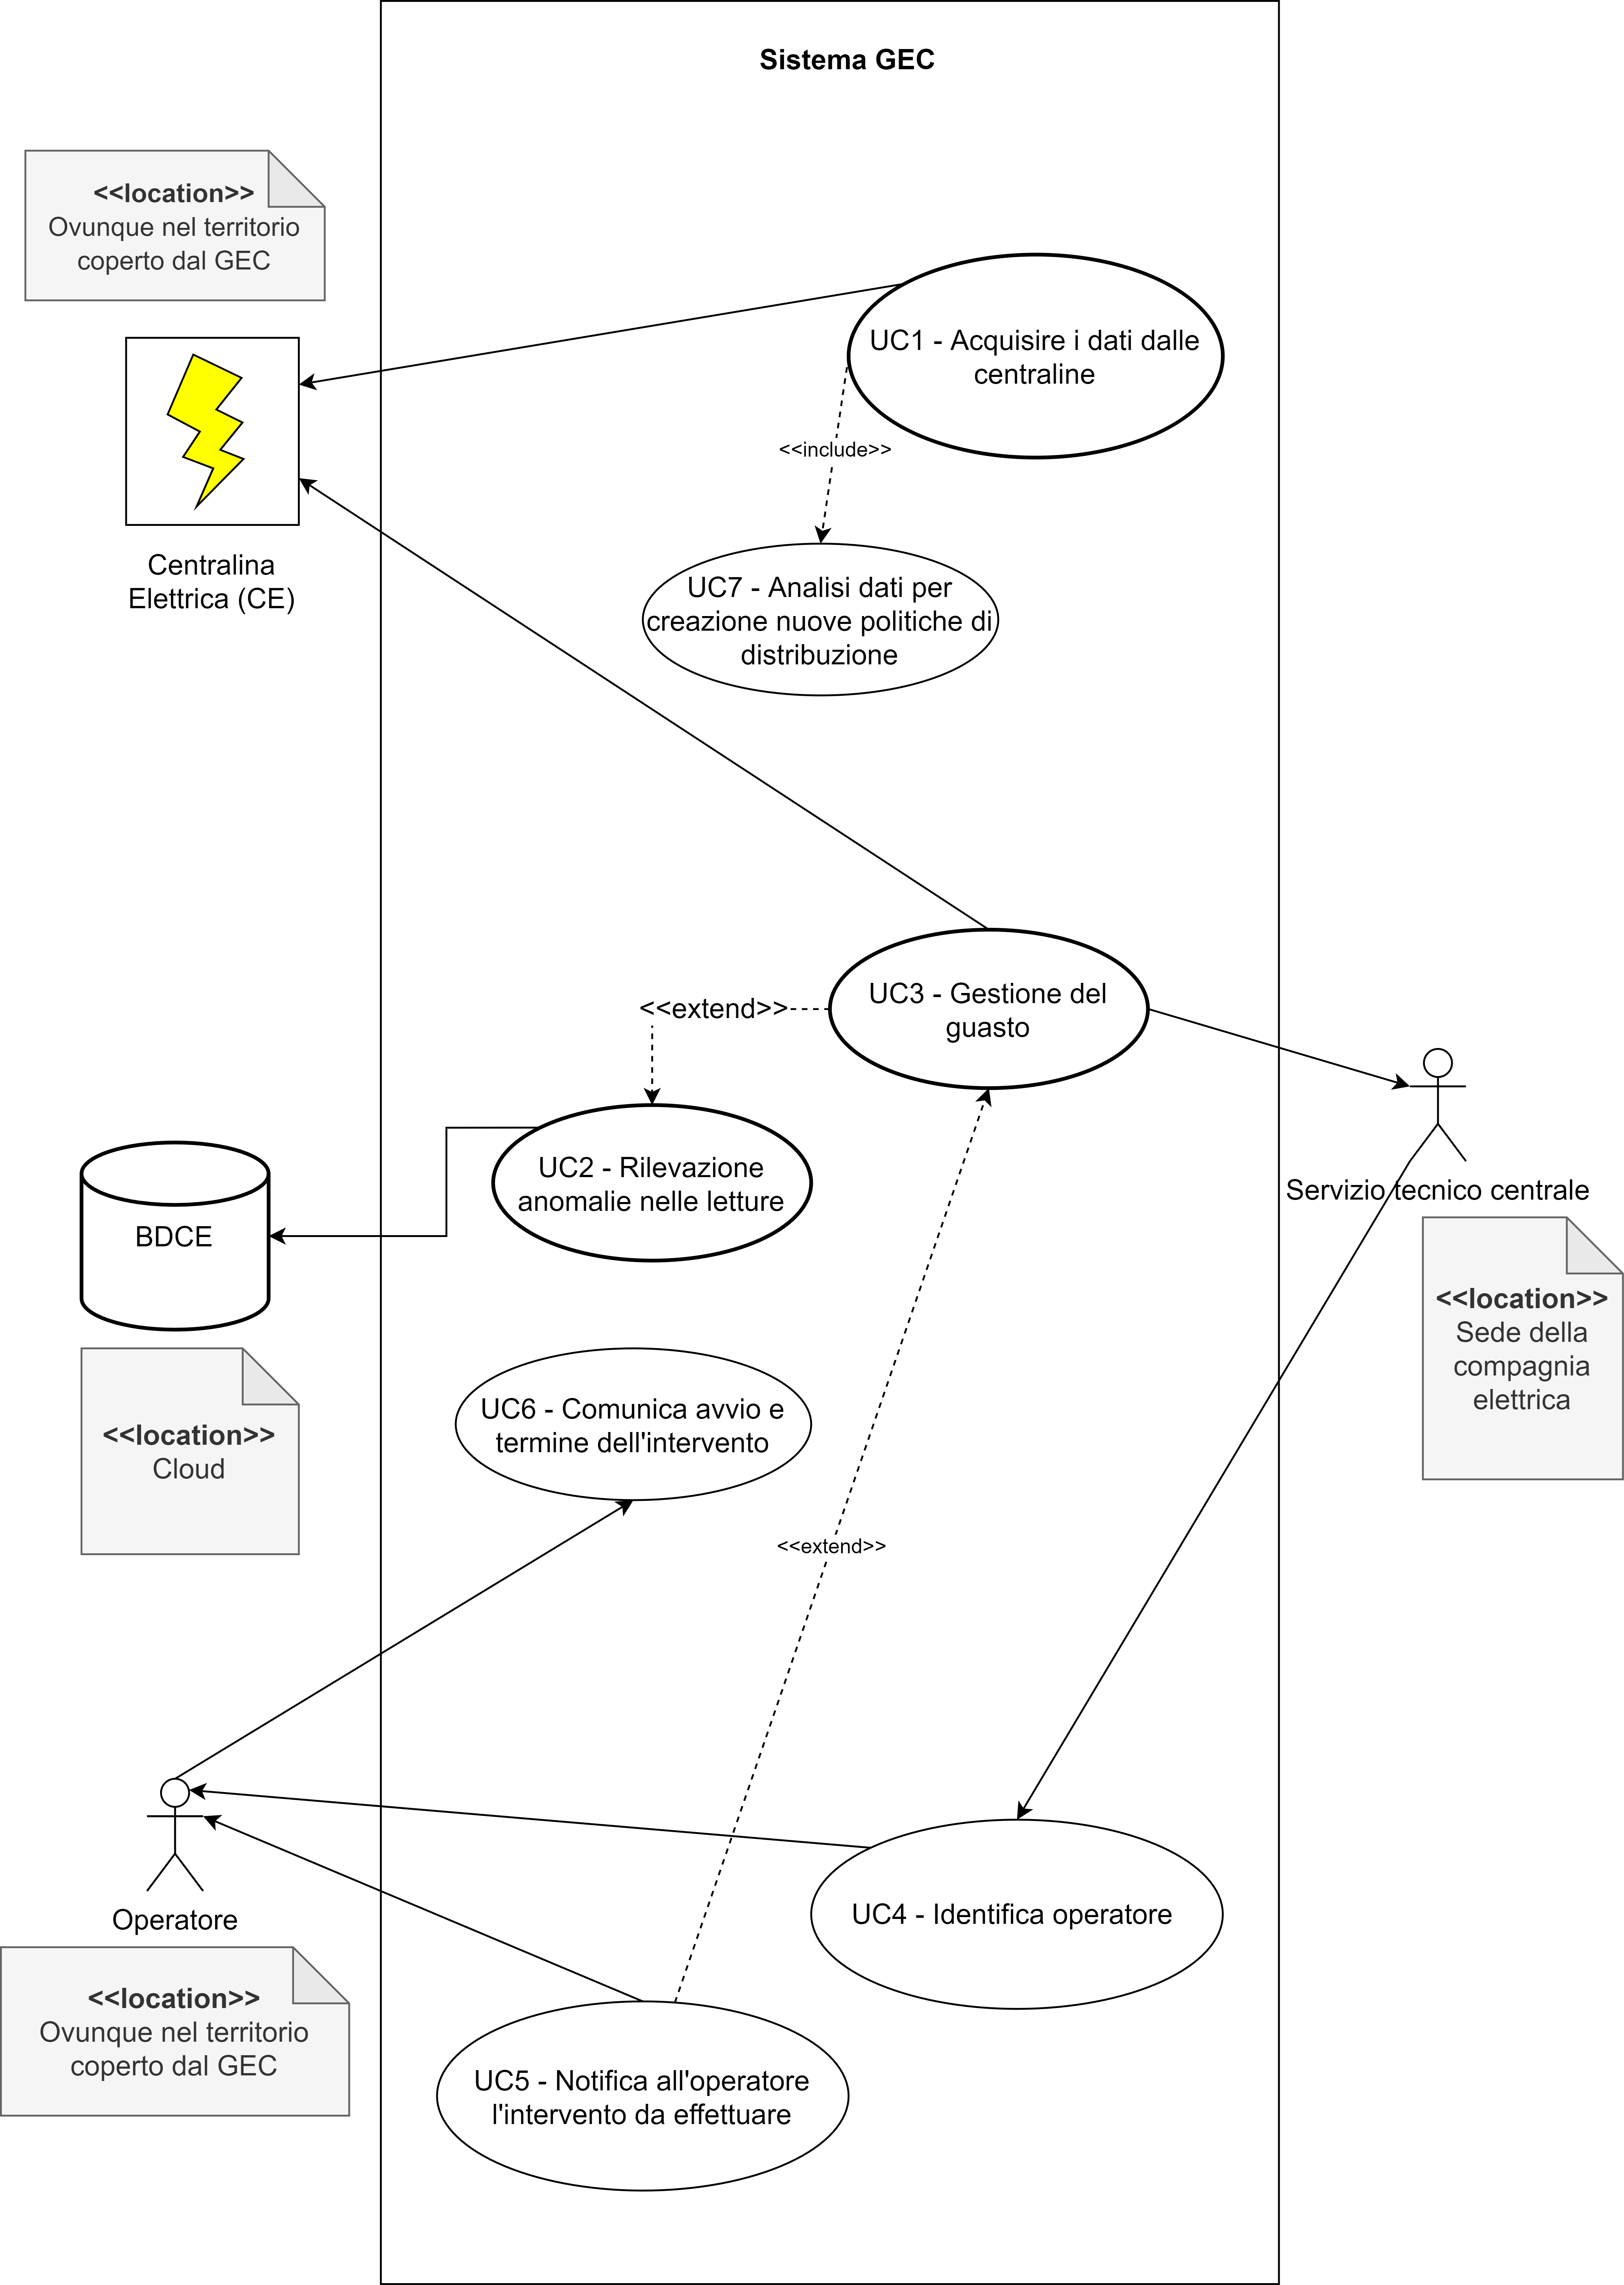
\includegraphics[width=\textwidth, height=0.85\textheight, keepaspectratio=true]{use_cases_diagram.png}
		\end{center}
	\end{frame}

	\subsection{Diagrammi delle attività}\label{activity_diagram}
		\begin{frame}[allowframebreaks]
		\frametitle{\nameref{use_cases_diagram}}
		\begin{block}{\nameref{use_cases_diagram}}
			\begin{itemize}
				\item ADUC1 - Acquisire dati centraline
				\item ADUC2 - Rilevazione anomalie nelle letture
				\item ADUC3 - Gestione dell'anomalia
				\item ADUC4 - Identifica operatore
				\item ADUC5 - Notifica all'operatore l'intervento da effettuare
				\item ADUC6 - Comunica avvio e termine dell'intervento
				\item ADUC7 - Analisi dati per creazione nuove politiche di distribuzione
			\end{itemize}
		\end{block}
	    \subsubsection{ADUC1 - Acquisire dati centraline}
		\begin{block}{ADUC1 - Acquisire dati centraline}
			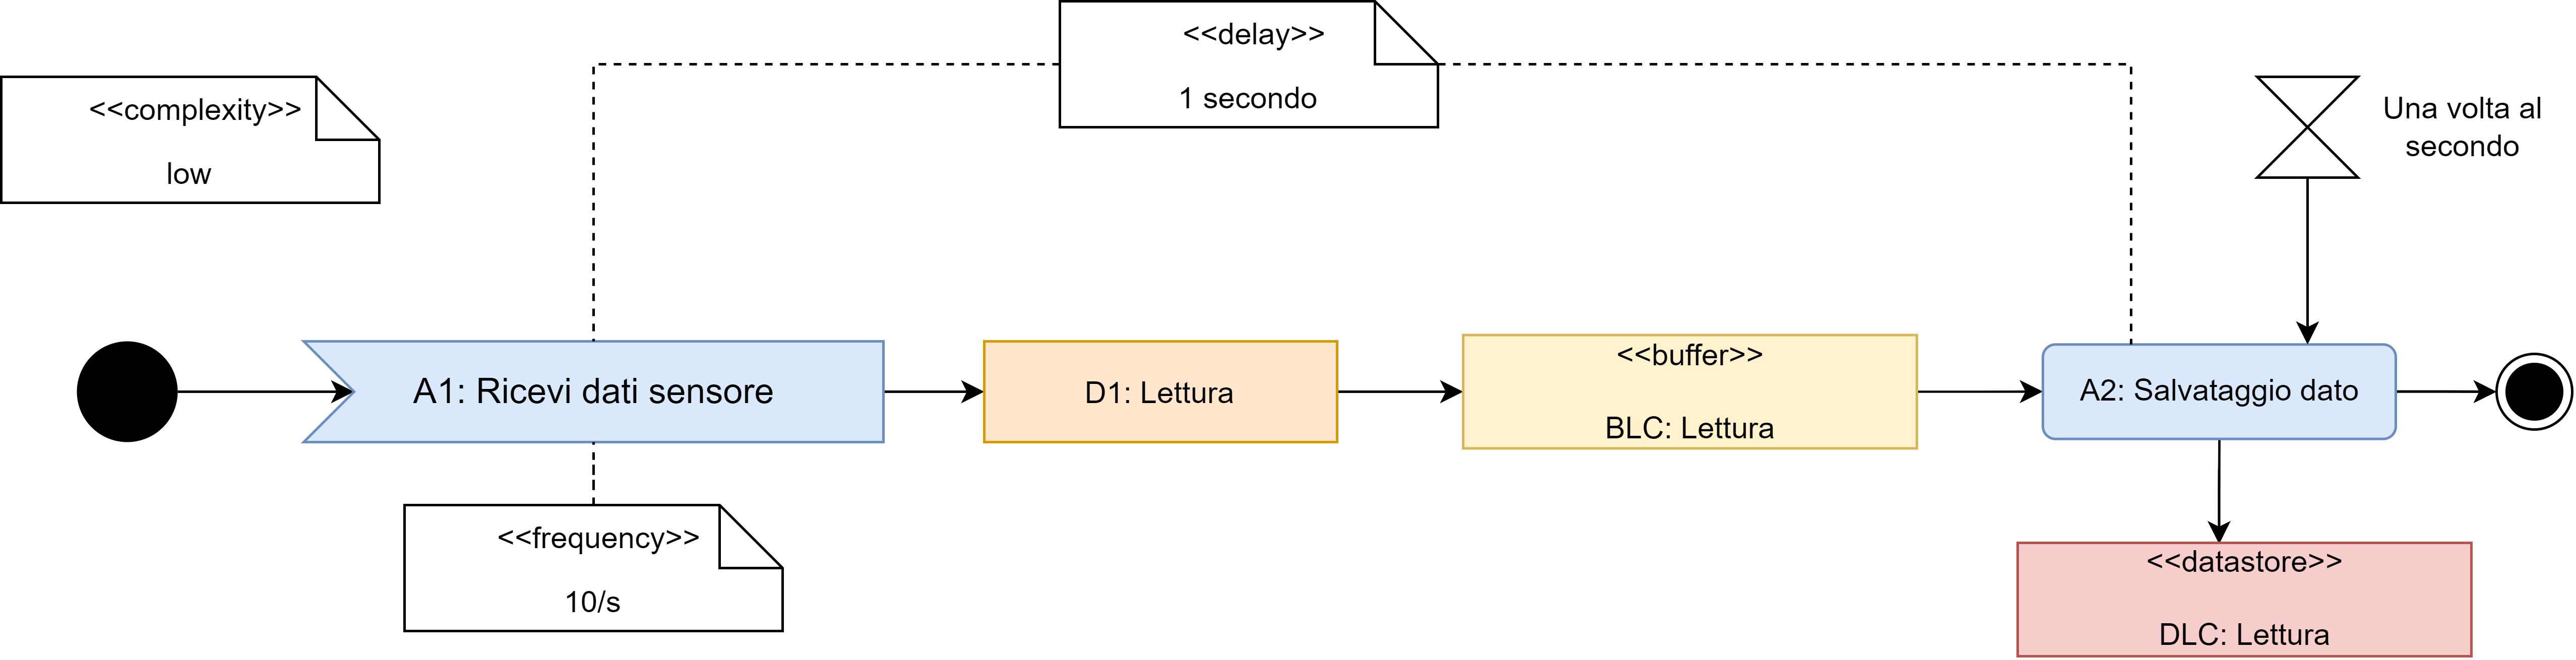
\includegraphics[width=\textwidth, height=0.85\textheight, keepaspectratio=true]{ADUC1.png}
		\end{block}
	\end{frame}
	
	
\end{document}
